\documentclass{article}

% 中文支持设置
\usepackage{xeCJK}
\setCJKmainfont{SimSun} % 设置中文字体为宋体,可根据系统字体调整
\setCJKsansfont{SimHei} % 设置中文无衬线字体为黑体
\setCJKmonofont{SimSun} % 设置中文等宽字体

% 页面设置
\usepackage[a4paper,top=2cm,bottom=2cm,left=3cm,right=3cm,marginparwidth=1.75cm]{geometry}

% 有用的包
\usepackage{amsmath}
\usepackage{graphicx}
\usepackage[colorlinks=true, allcolors=blue]{hyperref}

% 中文标签设置
\renewcommand{\abstractname}{摘要}
\renewcommand{\contentsname}{目录}
\renewcommand{\listfigurename}{插图目录}
\renewcommand{\listtablename}{表格目录}
\renewcommand{\refname}{参考文献}
\renewcommand{\indexname}{索引}
\renewcommand{\figurename}{图}
\renewcommand{\tablename}{表}
\renewcommand{\appendixname}{附录}

\title{一篇论文}
\author{我}
\usepackage{hyperref}
\begin{document}
\maketitle

\begin{abstract}
这是一个摘要
\end{abstract}

\section{引言}

您的引言在这里!只需开始编写您的文档并使用重新编译按钮查看更新的PDF预览。下面列出了常用命令和功能的示例,以帮助您入门。

一旦您熟悉了编辑器,您可以在Overleaf菜单中找到各种项目设置,该菜单可通过编辑器最左上角的按钮访问。要查看教程、用户指南和更多文档,请访问我们的\href{https://www.overleaf.com/learn}{帮助库},或前往我们的计划页面\href{https://www.overleaf.com/user/subscription/plans}{选择您的计划}。

\section{一些入门示例}

\subsection{如何创建章节和小节}

只需使用章节和小节命令,就像在这个示例文档中一样!使用Overleaf,所有格式和编号都会根据您选择的模板自动处理。如果您使用可视化编辑器,您也可以通过编辑器工具栏中的按钮创建新的章节和小节。

\subsection{如何包含图形}

首先,您必须使用文件树菜单中的上传链接从计算机上传图像文件。然后使用includegraphics命令将其包含在文档中。使用figure环境和caption命令为您的图形添加编号和标题。请参见本节中图\ref{fig:frog}的代码示例。

请注意,考虑到周围的文本以及可能附近的其他图形或表格,您的图形将自动放置在最合适的位置。您可以在这篇关于\href{https://www.overleaf.com/learn/how-to/Including_images_on_Overleaf}{在Overleaf上包含图像}的帮助文章中了解更多关于向文档添加图像的信息。

\begin{figure}
\centering
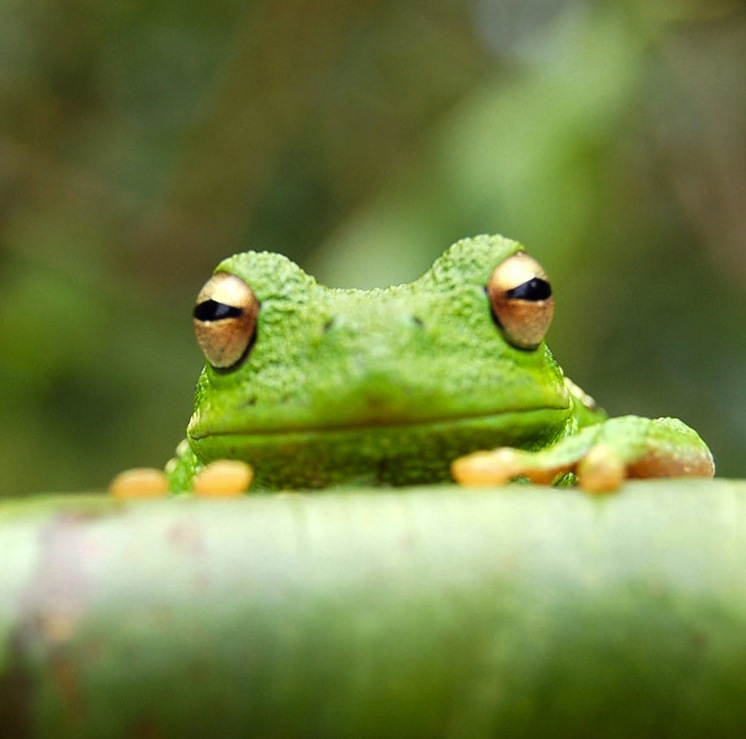
\includegraphics[width=0.25\linewidth]{frog.jpg}
\caption{\label{fig:frog}这只青蛙是通过文件树菜单上传的。}
\end{figure}

\subsection{如何添加表格}

使用table和tabular环境创建基本表格——例如表~\ref{tab:widgets}。更多信息,请参见这篇关于\href{https://www.overleaf.com/learn/latex/tables}{表格}的帮助文章。

\begin{table}
\centering
\begin{tabular}{l|r}
项目 & 数量 \\\hline
小部件 & 42 \\
小工具 & 13
\end{tabular}
\caption{\label{tab:widgets}示例表格。}
\end{table}

\subsection{如何添加注释和跟踪更改}

可以通过高亮显示一些文本并点击编辑器窗格右上角的"添加注释"来为您的项目添加注释。要查看现有注释,请点击上方工具栏中的审阅菜单。要回复注释,请点击注释右下角的回复按钮。当您暂时完成审阅时,可以通过点击工具栏上的名称来关闭审阅窗格。

跟踪更改功能在我们所有的\href{https://www.overleaf.com/user/subscription/plans}{高级计划}中都可用,可以使用审阅窗格顶部的选项来开启或关闭。跟踪更改允许您跟踪对文档所做的每一项更改,以及进行更改的人员。

\subsection{如何添加列表}

您可以制作自动编号的列表……

\begin{enumerate}
\item 像这样,
\item 也像这样。
\end{enumerate}
……或项目符号……
\begin{itemize}
\item 像这样,
\item 也像这样。
\end{itemize}

\subsection{如何编写数学公式}

\LaTeX{}在排版数学公式方面表现出色。设$X_1, X_2, \ldots, X_n$是一个独立同分布的随机变量序列,其中$\text{E}[X_i] = \mu$和$\text{Var}[X_i] = \sigma^2 < \infty$,设
\[S_n = \frac{X_1 + X_2 + \cdots + X_n}{n}
      = \frac{1}{n}\sum_{i}^{n} X_i\]
表示它们的均值。那么当$n$趋于无穷大时,随机变量$\sqrt{n}(S_n - \mu)$在分布上收敛到正态分布$\mathcal{N}(0, \sigma^2)$。


\subsection{如何更改页边距和纸张大小}

通常您使用的模板会为该用例正确设置页边距和纸张大小。例如,如果您使用期刊出版商提供的期刊文章模板,该模板将根据他们的要求进行格式化。在这些情况下,最好不要直接更改页边距。

但是,如果您使用的是更通用的模板(如这个模板),并且想要更改页边距,常见的方法是通过geometry包。您可以在此示例文件顶部的前言中找到加载的geometry包,如果您想了解更多关于如何调整设置的信息,请访问这篇关于\href{https://www.overleaf.com/learn/latex/page_size_and_margins}{页面大小和页边距}的帮助文章。

\subsection{如何更改文档语言和拼写检查设置}

Overleaf支持许多不同的语言,包括在一个文档中使用多种不同的语言。

要配置文档语言,只需编辑此示例项目顶部前言中提供给babel包的选项。要了解更多不同选项,请访问这篇关于\href{https://www.overleaf.com/learn/latex/International_language_support}{国际语言支持}的帮助文章。

要更改拼写检查语言,只需打开编辑器窗口左上角的Overleaf菜单,向下滚动到拼写检查设置,并相应调整。

\subsection{如何添加引用和参考文献列表}

您可以简单地上传一个包含BibTeX条目的\verb|.bib|文件,该文件可以使用JabRef等工具创建。然后您可以引用其中的条目,就像这样:\cite{greenwade93}。只需记住指定参考文献样式以及\verb|.bib|文件的文件名。您可以在\href{https://www.overleaf.com/help/97-how-to-include-a-bibliography-using-bibtex}{这里找到视频教程}来了解更多关于BibTeX的信息。

如果您有\href{https://www.overleaf.com/user/subscription/plans}{升级账户},您也可以通过文件树中的上传菜单直接将您的Mendeley或Zotero库导入为\verb|.bib|文件。

\subsection{祝您好运!}

我们希望您觉得Overleaf有用,并且请查看我们的\href{https://www.overleaf.com/learn}{帮助库}获取更多教程和用户指南!如果您有任何反馈,请使用Overleaf菜单底部的\textbf{联系我们}链接,或使用\url{https://www.overleaf.com/contact}的联系表单。

\bibliographystyle{alpha}
\bibliography{sample}

\end{document}
